\setAuthor{Andres Laan}
\setRound{lahtine}
\setYear{2010}
\setNumber{G 3}
\setDifficulty{4}
\setTopic{Dünaamika}

\prob{Veerev silinder}
\begin{wrapfigure}[7]{r}{0.3\textwidth}
	\vspace{-10pt}
	\hspace{-8pt}
	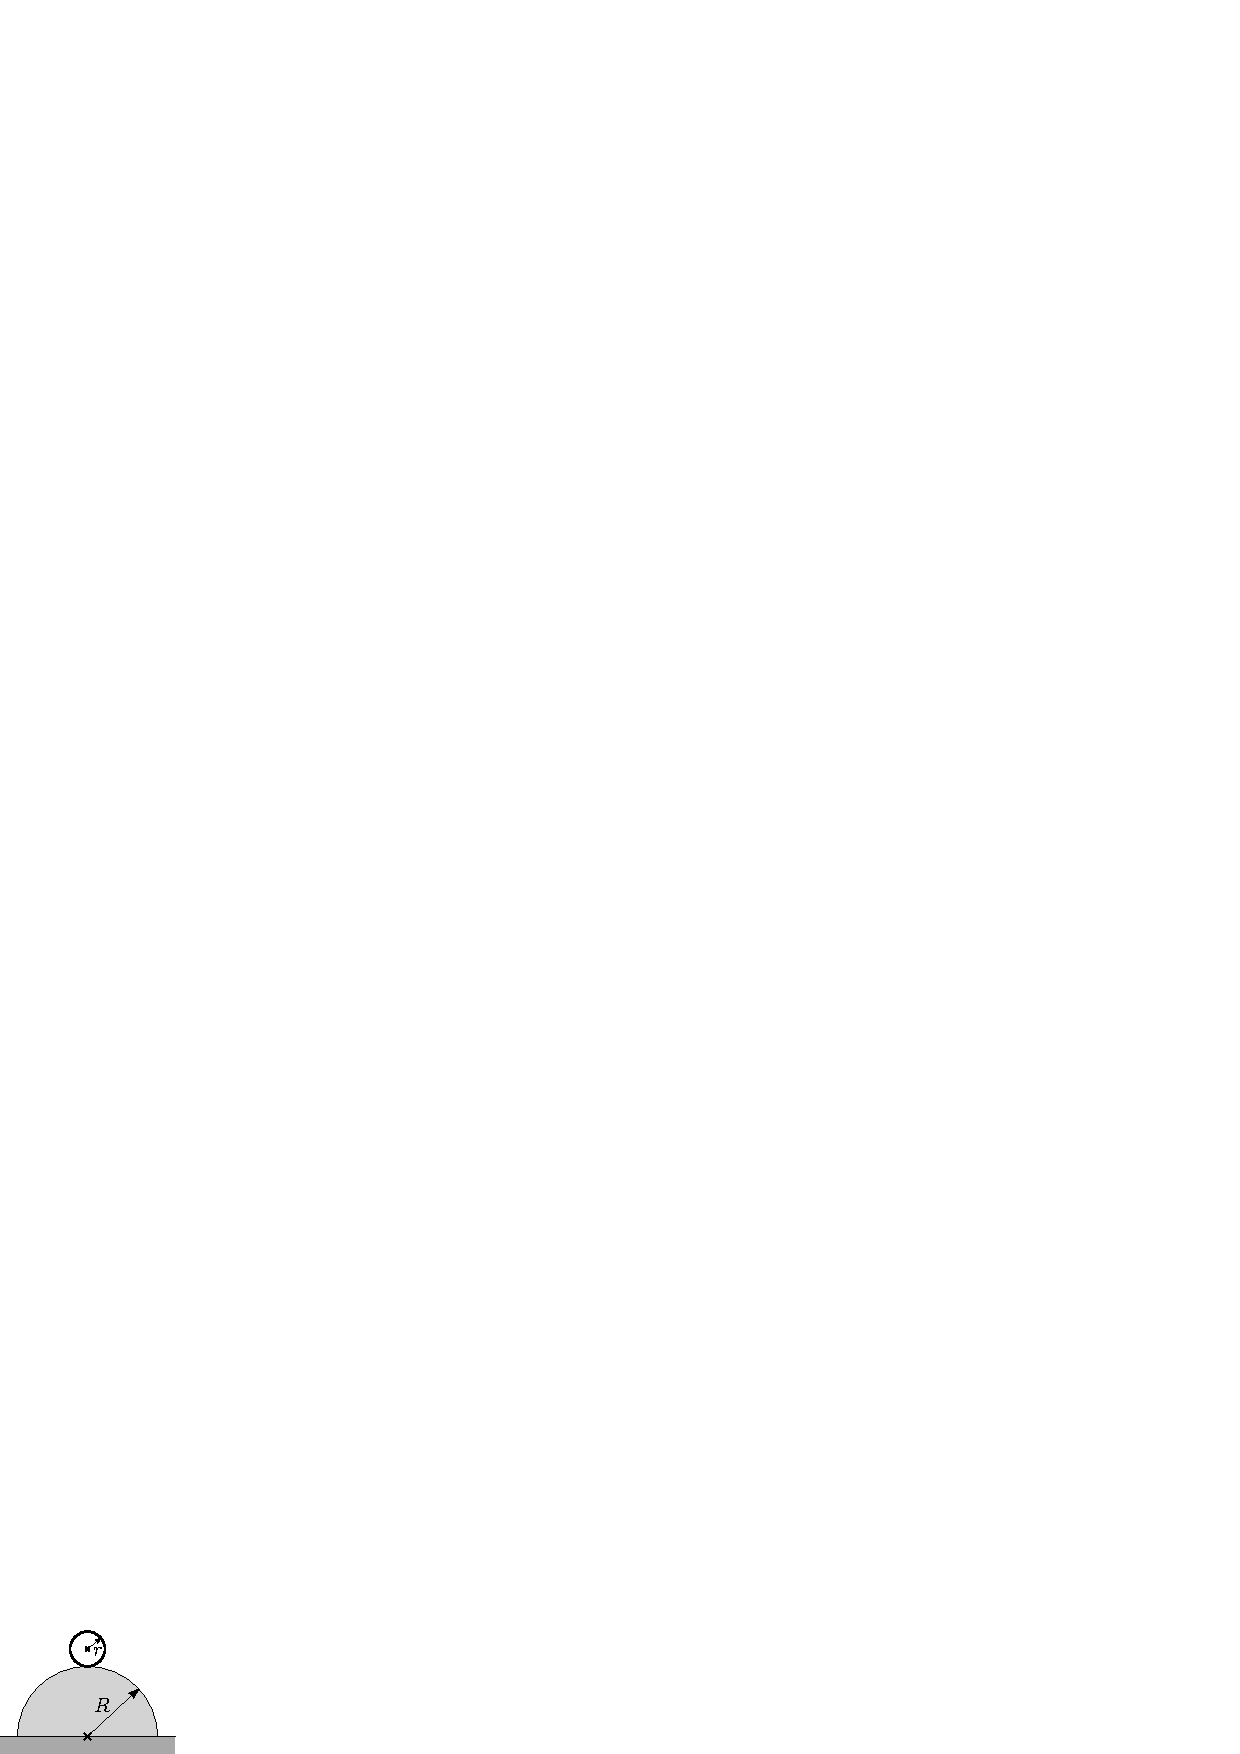
\includegraphics[width=\linewidth]{2010-lahg-03-silindri_joonis_ipe}
\end{wrapfigure}

Alusele kinnitatud poolsilindril raadiusega $R$
lebab selle kõrgeimas punktis seest tühi silinder
raadiusega $r$. Ühel hetkel nihkub keha veidi tasakaalust välja ja hakkab selle tulemusel libisemiseta veerema (hõõrdetegur on väga suur). Leidke, kui kõrgel aluse kohal keha
poolsilindri pinnast eraldub. \emph{Vihje:} kui veereva silindri mass on $m$ ja
ta masskese liigub kiirusega $v$, on ta kineetiline energia $m v^2$ (ilma
kordajata $\frac12$!).

\hint
Eraldumiskõrgust on kõige mugavam leida jõudude tasakaalust silindri keskpunkti radiaalsihis. Lisaks kehtib energia jäävuse seadus.

\solu
Eraldumiskõrgust on kõige lihtsam arvutada kasutades jõudude tasakaalu. 
Nii kaua kui veerev keha on alusega kontaktis, mõjub talle toereaktsioon. 
Pinnalt eraldumise punktis muutub toereaktsioon nulliks ja raskusjõu raadiusesihiline 
komponent saab võrdseks kesktõmbekiirendusega. Seega
\[
\frac{mv^2}{R+r}=mg\cos\alpha,
\]
kus $\alpha$ on pinna kaldenurk eraldumispunktis (mis asub kõrgusel $H=(r+R)\cos\alpha$). 
Vastav kiirus on leitav energia jäävuse seadusest ehk
võrdsustades gravitatsioonienergia muudu kulg- ja pöördliikumise kineetilise energiaga:
\[
mg(R+r-H)=mv^2.
\]
Elimineerides eelnevaist võrrandeist $\cos\alpha$, saame tulemuseks $H=(r+R)/2$.
\probend